\documentclass{beamer}
\usepackage[italian]{babel}
\usepackage{graphicx}
\usepackage[utf8x]{inputenc}

\title[Borgovolley 2017/2018]{Riunione Tecnica Borgovolley 2017/2018}
%\titlegraphic{\includegraphics[width=15mm]{../relazione/img/Sigillo.pdf}}
\date[24 Agosto 2017]{}

\usetheme{CambridgeUS}

\usecolortheme{dolphin}
\setbeamertemplate{navigation symbols}{}

\begin{document}

\begin{frame}
\maketitle
\end{frame}

\begin{frame}
\frametitle{Mission}
\begin{block}{L'obiettivo dell'A.S.D. Borgovolley Fidenza}
Contribuire alla \alert{crescita} tecnica, mentale e fisica dei giovani del \alert{territorio}, trasmettendo \alert{gioia} e passione per lo sport!
\end{block}
\end{frame}

\section{Organigramma 2017}
\begin{frame}
\frametitle{Organigramma 2017}
\begin{block}{Direzione Societaria}
\begin{itemize}
\item[-]Responsabile Società: Dado e Gabriella;
\item[-]Direttore Tecnico Squadre: Luciana Do Carmo;
\item[-]Direttore Tecnico Minivolley: Gabriella;
\item[-]Direttore Sportivo: Dado;
\item[-]Responsabile Sponsor: Silvia e Gabriella;
\item[-]Responsabile visite mediche: Gabriella;
\end{itemize}
\end{block}
\end{frame}

\begin{frame}
\frametitle{Organigramma 2017}
\begin{block}{Squadre e Allenatori}
\begin{itemize}
\item[-]Borgovolley Team (2 Div): \textbf{Luciana}, Carlo, Fabio;
\item[-]Borgovolley U18: \textbf{Luciana}, Carlo, Fabio;
\item[-]Borgovolley U16: \textbf{Umberto}, Lollo, Silvia;
\item[-]Borgovolley U14: \textbf{Umberto};
\item[-]Borgo Manu (U13/14): \textbf{Manu};
\item[-]Borgovolley 13: \textbf{Dado}, Silvia;
\item[-]Borgovolley 12: \textbf{Dado}.
\end{itemize}
\end{block}

\begin{block}{Attività da definire}
Juri, Lollo e Pette.
\end{block}
\end{frame}

\begin{frame}
\frametitle{Organigramma 2017}
\begin{block}{Attività Promozionale}
\begin{itemize}
\item[-]Psicomotricità: Benedetta;
\item[-]Corso Minivolley: Gabriella;
\item[-]3 gruppi amatori: Responsabile Juri;
\item[-]Attività scolastica: Luciana, Barbara, Michele.
\end{itemize}
\end{block}
\end{frame}


\section{Attività}


\begin{frame}
\frametitle{Inizio Attività}
\begin{itemize}
\item[-]Borgovolley Team 2a Div e U18: 4/9, ore 18.00;
\item[-]Borgovolley U16: 4/9, ore 18.30, Collodi;
\item[-]Borgovolley U14: 4/9, ore 16.30, Collodi;
\item[-]Borgo Manu U13 e 14: 11/9;
\item[-]Borgovolley 13: 11/9;
\item[-]Borgovolley 12: 11/9;
\item[-]Psicomotricità: 18/9;
\item[-]Corso Minivolley: 19/9.
\end{itemize}
\end{frame}


\begin{frame}
\frametitle{Spazi e Palestre}
\begin{center}
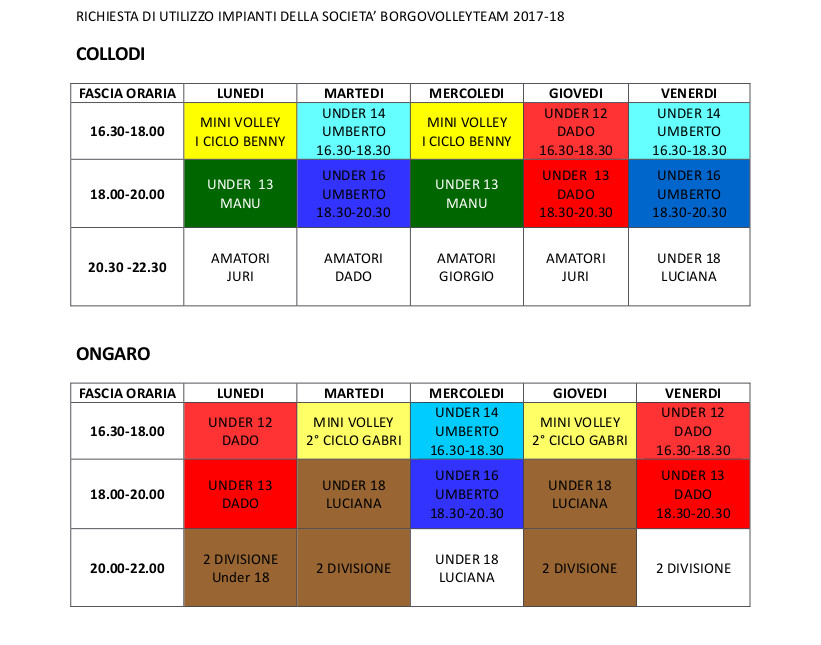
\includegraphics[scale=0.47]{palestre2017-18.jpg}
\end{center}
\end{frame}


\begin{frame}
\frametitle{Calendario Riunioni}
\begin{itemize}
\item[-]Borgovolley Team 2a Div e U18: 4/9 ore 20.30, Palazzetto (*);
\item[-]Borgovolley U16: 8/9 ore 20.30, palestra Collodi;
\item[-]Borgovolley U14: 11/9 ore 20.30, Palazzetto (*);
\item[-]Borgo Manu U13 e U14: 6/9 ore 20.30, Palazzetto (*);
\item[-]Borgovolley 13: 7/9 ore 20.30,  Palazzetto (*);
\item[-]Borgovolley 12: 7/9 ore 19.30, Palazzetto (*).
\end{itemize}

(*) da confermare
\end{frame}


\begin{frame}
\frametitle{Altre Attività ed Impegni}
\begin{itemize}
\item[-]Corso Defibrillatore 4/11/2017, Salsomaggiore;
\item[-]Controllo e consegna materiale entro fine settembre;
\item[-]Presentazione Società da definire;
\item[-]Riunione Tecnica Mensile, ultimo mercoledì del mese.
\end{itemize}

\begin{block}{Eventuale partecipazioni tornei di settembre}
\begin{itemize}
\item[-]Busseto 16/9/2017, U16, Minivolley e U12;
\item[-]Collecchio 8-9-10/9/2017, Minivolley, U12 e U13.
\end{itemize}
\end{block}
\end{frame}

\section{Regolamento}


\begin{frame}
\frametitle{Regolamento Atlete}
\begin{itemize}
\item[-]Conoscenza ed accettazione del Regolamento;
\item[-]Assenze/Ritardi allenamenti e partite;
\item[-]Abbigliamento;
\item[-]Visite mediche e infortuni;
\item[-]Corretto utilizzo spazi di attrezzature e spazi;
\item[-]Etica;
\item[-]Conoscenza Regole Tesseramento FIPAV.
\end{itemize}
\end{frame}


\begin{frame}
\frametitle{Regolamento Allenatori}
\begin{itemize}[<+->]
\item[-]Far rispettare il Regolamento Atlete;
\item[-]Mantenere fede ai valori etico/morali verso atleti e genitori;
\item[-]Promuovere una sana competizione;
\item[-]Costruire un progetto che sia prima educativo e poi agonistico;
\item[-]Essere esempi per le atlete;
\item[-]Partecipare alle iniziative della Società;
\item[-]Mantenere un clima sereno e favorevole alle attività in un ambiente sicuro.
\end{itemize}

\pause
\begin{block}{Sinergia e Rispetto}
Mi piacerebbe sentire allenatori che lavorano sul materiale che hanno, se ci sono difficoltà ci si aiuta, parlandone nelle riunioni tecniche.
\end{block}
\pause
\begin{alertblock}{Riservatezza}
Ognuno all'interno della società deve mantenere il proprio ruolo. 
\end{alertblock}
\end{frame}

\begin{frame}
\frametitle{Formazione Squadre}

\end{frame}

\end{document}